%%%%%%%%%%%%%%%%%%%%%%%%%%%%%%%%%%%%%%%%%%%%%%%%%%%%%%%%%%%%%%%%%%%%%%%%%%%%%%%%
%
%	OVERVIEW OF GPU ARCHITECTURE
%
%%%%%%%%%%%%%%%%%%%%%%%%%%%%%%%%%%%%%%%%%%%%%%%%%%%%%%%%%%%%%%%%%%%%%%%%%%%%%%%%

\begin{figure}
	\centering
	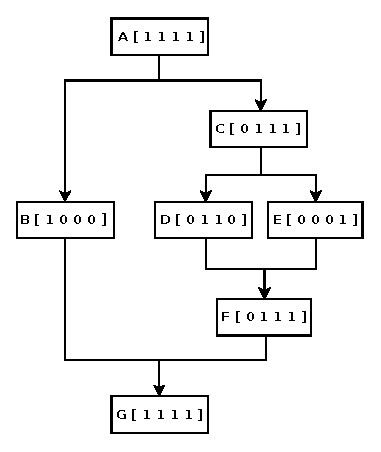
\includegraphics[width=8cm]{control-flow-graph}
	\caption{A sample control flow graph to understand branch divergence. Each block in the graph depicts the name of a basic block followed by a 4 bit vector show the status of different threads while executing that basic block. The $i^{th}$ bit represents the state of the $i^{th}$ thread.
	\label{fig:control-flow-graph}} 
\end{figure}
The Graphics Processing Unit (GPU) is a specialized unit for graphics applications. Early graphics applications had very little control flow, and the overwhelming goal of a designer was to maximize floating-point throughput by exploiting data-parallelism. This led to the development of a highly-parallel architecture where numerous processors share the same global graphics memory interface, and each processor is comprised of a multi-threaded pipeline sharing the same fetch and decode stages but different execution pipelines and registers. The emphasis on functional units over control is a distinctive feature of the GPU as it performs best on a Single-Program Multiple Data (SPMD) task.


\subsection*{Branch Divergence}
\label{sec:branch-divergence-description}
A typical GPU consists of a pipeline which executes a group of threads in lock-step, called \textsl{warp}. Since the warp is constrained to execute the same instruction, a unique branch penalty occurs when all the threads do not resolve in the same direction, called \textsl{branch divergence}. 

To illustrate the phenomenon, let us consider a program with a control-flow as shown in Fig. \ref{fig:control-flow-graph}. Here, a warp is assumed to have four threads, and each thread executes the branch instructions A and C on their private data. The way a certain thread resolved at a branch can be derived from its mask in the next instruction. For instance, the first thread resolves towards B at A, as its mask is 1 in B but 0 in C.Since all the threads are constrained to execute the same instruction, some threads remain inactive while others are active (when executing D, only the second and third threads are active). This leads to a loss in execution cycles compared to the ideal case when all the threads are active in a warp. Our goal is to measure the share of such performance degradation due to branches not central to the algorithm.

